% !TEX encoding = UTF-8 Unicode
\documentclass[aodsor,preprint]{imsart}
\usepackage{amsthm,amsmath,amssymb}
\usepackage{graphicx}
\usepackage[authoryear,round]{natbib}
\usepackage[colorlinks,citecolor=blue,urlcolor=blue]{hyperref}
\usepackage[utf8]{inputenc}
%\usepackage{ngerman}
\usepackage{listings}
\usepackage{xcolor}
\usepackage{csquotes}

\lstset{
  basicstyle=\ttfamily\small,
  numbers=left,
  numberstyle=\tiny,
  stepnumber=1,
  numbersep=5pt,
  backgroundcolor=\color{white},
  showspaces=false,
  showstringspaces=false,
  showtabs=false,
  frame=single,
  captionpos=t,
  abovecaptionskip=1em,
  breaklines=true,
  breakatwhitespace=false,
  keywordstyle=\color{blue},
  commentstyle=\color{green!50!black},
  stringstyle=\color{orange},
  language=R
}

% settings
%\pubyear{2005}
%\volume{0}
%\issue{0}
%\firstpage{1}
%\lastpage{8}
%\arxiv{arXiv:0000.0000}


\numberwithin{equation}{section}
\theoremstyle{plain}
\newtheorem{thm}{Theorem}[section]
\newtheorem{lemma}[thm]{Lemma}
\newtheorem{corollary}[thm]{Corollary}
\newtheorem{remark}[thm]{Remark}
\newtheorem*{remark*}{Remark}

% customize math operators
\newcommand{\E}{{\mathbb E}}


\begin{document}

\begin{frontmatter}
\title{Das Gesetz der Großen Zahlen: Beweismethoden,
Vergleiche und Anwendungsfälle}
\runtitle{Das Gesetz der Großen Zahlen}


\begin{aug}
\author{\fnms{Valentino} \snm{Galliano}\ead[label=e1]{a12149634@unet.univie.ac.at}}


\runauthor{Valentino Galliano}

\affiliation{University of Vienna}

\end{aug}

\begin{abstract}
    Diese Arbeit untersucht das Gesetz der Großen Zahlen (GGZ), ein zentrales Konzept der Wahrscheinlichkeitstheorie.
    Nach einer historischen Einordnung des GGZ in den letzten Jahrhunderten wird zwischen dem starken und dem schwachen GGZ formal unterschieden.
    Die Arbeit präsentiert die mathematischen Grundlagen beider Gesetze und beschreibt die Unterscheidung zwischen Konvergenz in Wahrscheinlichkeit (schwaches GGZ) und fast sicherer Konvergenz (starkes GGZ).
    Darüber hinaus stellt die Arbeit verschiedene Beweismethoden für das schwache GGZ vor, etwa mithilfe der Tschebyscheff- und Markow-Ungleichung, sowie den Zusammenhang zum zentralen Grenzwertsatz und zum Gesetz des iterierten Logarithmus.
    Um die praktische Anwendbarkeit des GGZ zu untersuchen, geht diese Arbeit auf verschiedene Anwendungsbereiche an und diskutiert darauffolgend die Grenzen und Gegenbeispiele des GGZ.
    Ziel der Arbeit, die mathematischen Grundlagen, unterschiedliche Beweismethoden, praktische Anwendungsfälle und Limitationen des GGZ darzustellen.
\end{abstract}

\begin{keyword}[class=MSC]
\kwd[Primary ]{60K35}
\kwd{60K35}
\kwd[; secondary ]{60K35}
\end{keyword}

\begin{keyword}
\kwd{sample}
\kwd{\LaTeXe}
\end{keyword}

\end{frontmatter}

\section{Einleitung}
\label{sec:einleitung}
Das Gesetz der Großen Zahlen (GGZ) ist ein grundlegendes Konzept in der Statistik und Wahrscheinlichkeitstheorie.
Es beschreibt die Stabilisierung von Mittelwerten bei einer zunehmenden Anzahl von Zufallsexperimenten oder Stichproben \citep{degroot2021}.
Dieses Gesetz bildet die Grundlage für viele statistische und stochastische Methoden in der Mathematik und wird nicht nur in der Theorie, sondern auch in sämtlichen praktischen Bereichen angewendet, wie z.B. in Simulationen und in der Analyse großer Datenmengen.


Ein zentraler Punkt ist die Unterscheidung zwischen dem starken und dem schwachen GGZ.
Das schwache GGZ besagt, dass der arithmetische Mittelwert einer Folge unabhängiger, identisch verteilter Zufallsvariablen mit wachsendem Stichprobenumfang in Wahrscheinlichkeit gegen den Erwartungswert konvergiert.
Das starke GGZ trifft eine stärkere Aussage: Es garantiert die fast sichere Konvergenz des arithmetischen Mittels gegen den Erwartungswert.
Dies bedeutet, dass der arithmetische Mittelwert mit einer Wahrscheinlichkeit von 1 gegen den Erwartungswert konvergiert.
Diese Unterscheidung ist essenziell für meine Arbeit, da sie sich vor allem auf die verschiedenen Beweise des schwachen GGZ konzentriert.
Diese Arbeit untersucht das schwache GGZ umfassend und grenzt es vom starken GGZ ab.
Darüber hinaus werden Beweise vertieft untersucht und die Beziehung zum zentralen Grenzwertsatz dargestellt.
Für diesen Zweck stützt sich die Arbeit auf eine Auswahl anerkannter Fachliteratur, insbesondere \citet{degroot2021, blitzstein2019, stoyanov2013}.

\newpage


\textbf{Beispiel: Münzwurf}

Ein klassisches Beispiel für das GGZ ist das wiederholte Werfen einer fairen Münze.
Sei \( X_i \in \{0,1\} \) die Zufallsvariable für Wurf \( i \). Der Wert 1 steht hier für \enquote{Kopf}. Dann ist \( \mu = \mathbb{E}[X_i] = 0{,}5 \) bei einer fairen Münze, und das GGZ garantiert:
\[
\frac{1}{n} \sum_{i=1}^n X_i \xrightarrow{\mathbb{P}} 0{,}5.
\]
Dies bedeutet, dass die beobachtete Wahrscheinlichkeit von \enquote{Kopf} bei wachsender Anzahl von Würfen gegen die wahre Wahrscheinlichkeit geht.
Selbstverständlich trifft diese Regel auch auf die Wahrscheinlichkeit von \enquote{Zahl} zu. 

Zur Veranschaulichung dieses Beispiels kann man auch eine einfache Computersimulation durchführen.
Das Ergebnis dieser Simulation in der Programmiersprache R sieht man in Abbildung \ref{fig:muenzwurf}.
Anhand dieser Simulation sieht man auch visuell, dass der empirische Mittelwert bei einer niedrigen Anzahl von Würfen noch sehr stark von dem Erwartungswert 0.5 abweicht.
Wenn man jedoch die Anzahl der Würfe erhöht (y-Achse), sinkt diese Abweichung und der empirische Mittelwert konvergiert gegen den echten Erwartungswert.


\begin{figure}[h!]
  \centering
  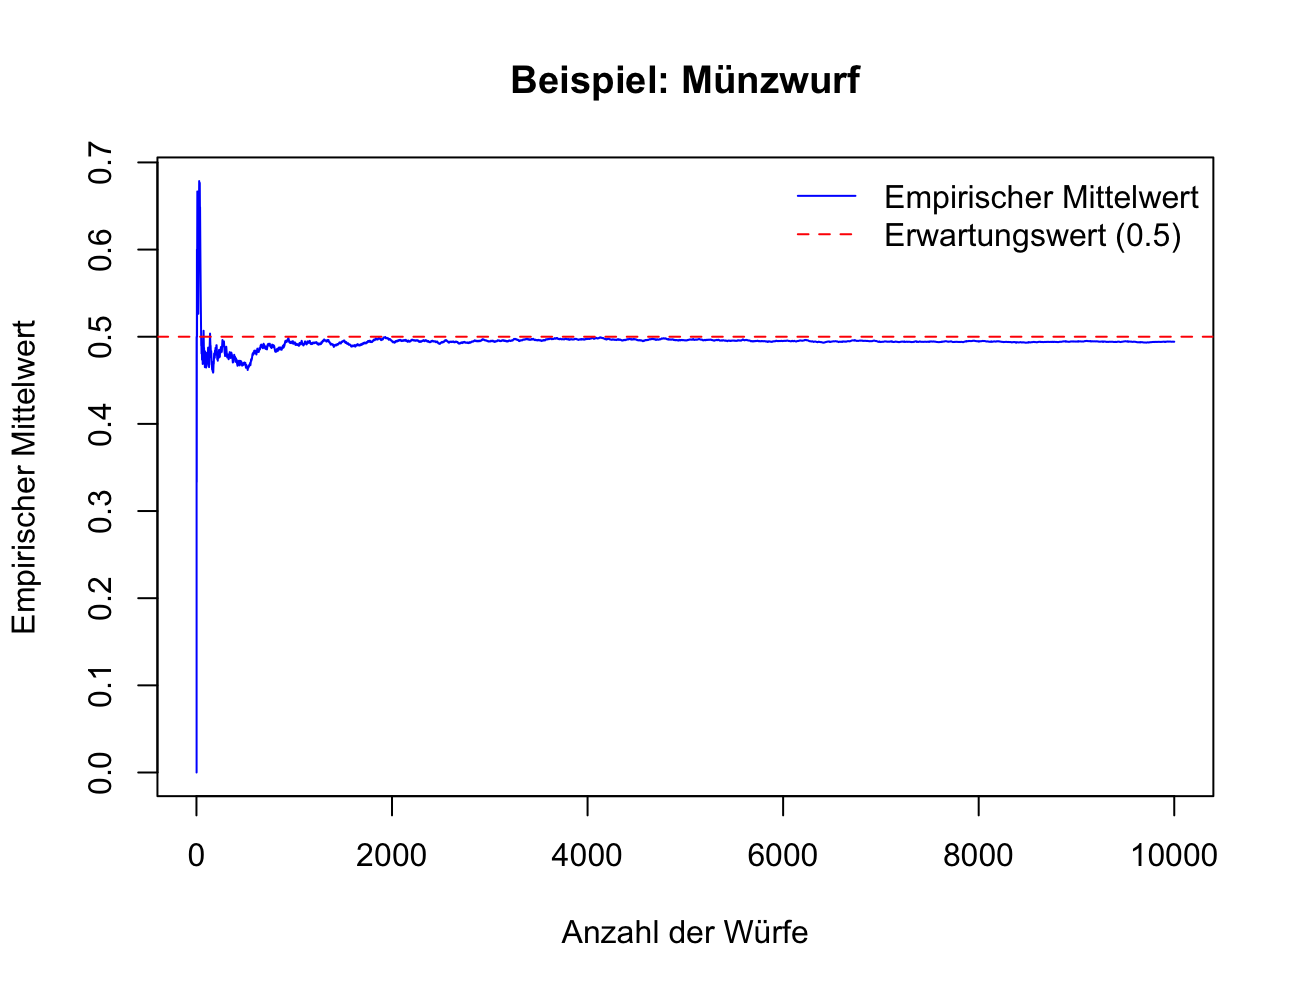
\includegraphics[width=0.9\textwidth]{Muenzwurf.png}
  \caption{Simulation eines Münzwurfs zur Veranschaulichung des Gesetzes der großen Zahlen}
  \label{fig:muenzwurf}
\end{figure}

\newpage

Die Struktur der Arbeit orientiert sich an dem folgenden Aufbau.
In Kapitel \ref{sec:hist} werden die historischen Entwicklungen des GGZ vorgestellt, sowie relevante Begriffe eingeführt.
In Kapitel \ref{sec:definitionen} erfolgt die Definition des GGZ und seiner Voraussetzungen, gefolgt von praktischen Anwendungen, sowie dem Vergleich zwischen dem starken und schwachen GGZ.

In Kapitel \ref{sec:beweismethoden} werden verschiedene Beweise des GGZ präsentiert.
Da der Fokus dieser Arbeit auf den Beweismethoden des schwachen GGZ liegt, werden diese detailliert in Unterkapitel \ref{sec:beweisschwach} vorgestellt.
Insbesondere wird auch der Bezug zum zentralen Grenzwertsatz und dem Gesetz des iterierten Logarithmus untersucht.
In Unterkapitel \ref{sec:beweisstark} wird danach das starke GGZ formal bewiesen.
In Kapitel \ref{sec:anwendung} werden sämtliche Anwendungsfälle des GGZ vorgestellt und die praktische Relevanz näher beschrieben.
In Kapitel \ref{sec:grenzen} werden einige Gegenbeispiele und bekannte Grenzen des GGZ dargestellt. 
Abschließend erfolgt eine Zusammenfassung dieser Arbeit in Kapitel \ref{sec:zusammenfassung}.
Die Onlineversion der Seminararbeit findet man auf GitHub. \footnote{\url{https://github.com/ValentinoGalliano/code-seminarbeit}}



\section{Historischer Überblick und Einordnung}
\label{sec:hist}
Die Geschichte des GGZ reicht bis ins 18. Jahrhundert zurück.
Daniel Bernoulli, Schweizer Mathematiker und Physiker, formulierte im Jahr 1713 ein Ergebnis \citep{bernoulli1713}, das heute als Vorläufer des GGZ gesehen wird.
Er zeigte, dass bei wiederholter Durchführung eines Zufallsexperiments sich die relative Häufigkeit eines Ereignisses seiner wahren Wahrscheinlichkeit nähert, wenn man die Anzahl der Versuche erhöht.
Bernoulli bewies analytisch auch, dass für unabhängige Bernoulli-Experimente die relative Häufigkeit des Erfolgs mit großer Wahrscheinlichkeit nahe bei der Erfolgswahrscheinlichkeit liegt.
Dieses Ergebnis wurde später von mehreren Autoren bestätigt und verallgemeinert \citep{poisson1837theorie, chebyshev1867}.


Erst Anfang des 20. Jahrhunderts etablierte sich in \citep{borel1909probabilites} die mathematische Fassung von \enquote{fast sicher}.
In der Wahrscheinlichkeitstheorie bedeutet \enquote{fast sicher}, dass ein Ereignis mit Wahrscheinlichkeit 1 eintritt.
Formal ausgedrückt ist also
\[\mathbb{P}(A) = 1,\]
wobei \( A \) das betrachtete Ereignis ist. Wichtig ist dabei anzumerken, dass diese Aussage nicht ausschließt, dass \( A \) in Ausnahmefällen trotzdem nicht eintritt. Der Grund dafür ist, dass auch Ereignisse mit Wahrscheinlichkeit 0 nicht unmöglich sind, sondern nur \enquote{fast nie} beobachtbar sind.
Diese Feststellung unterstreicht die wesentliche Bedeutung, in mathematischen Kontexten \enquote{sicher} von \enquote{fast sicher} zu unterscheiden.


Im 20. Jahrhundert wurde das GGZ durch Arbeiten von Mathematikern wie  Andrei Nikolajewitsch Kolmogorow und Émile Borel weiter formalisiert und erweitert.
Sie bewiesen das starke Gesetz der großen Zahlen unter allgemeinen Bedingungen und betonten somit die Bedeutung der \enquote{fast sicheren} Konvergenz.
Parallel dazu entwickelten sich im Laufe der Zeit auch abgeschwächte Formen des Gesetzes, etwa das schwache Gesetz der großen Zahlen.


Der historische Hintergrund des GGZ zeigt die zunehmende Forschung und Literatur im Bereich der Konvergenz und die erhöhte Bedeutung der mathematischen Präzision. Darüber hinaus sieht man auch, dass die Relevanz von unterschiedlichen Grenzwertsätzen in der mathematischen Theorie sowie Praxis immer mehr an Bedeutung gewonnen hat.

\section{Formale Definitionen}
\label{sec:definitionen}


In diesem Kapitel werden die notwendigen formalen Definitionen zum GGZ vorgestellt.


\subsection{Zufallsvariable}

\textbf{Definition:}
Eine \emph{Zufallsvariable} ist eine messbare Funktion \( X \colon \Omega \to \mathbb{R} \), die jedem Ergebnis \(\omega \in \Omega\) eines Zufallsexperiments eine reelle Zahl \(X(\omega)\) zuordnet.

Dabei ist \(\Omega\) der Ergebnisraum des Zufallsexperiments, und die Abbildung \(X\) erlaubt es, Ereignisse auf reelle Zahlen abzubilden und somit mithilfe der Wahrscheinlichkeitsrechnung zu analysieren.


\subsection{i.i.d. Zufallsvariablen}

\textbf{Definition:}
Eine Folge von Zufallsvariablen \( X_1, X_2, \dots, X_n \) heißt \emph{i.i.d.} (engl. \emph{independent and identically distributed}), wenn folgende zwei Bedingungen erfüllt sind:

\begin{itemize}
  \item \textbf{Unabhängigkeit:} Die Zufallsvariablen \( X_1, \dots, X_n \) sind stochastisch unabhängig, d.\,h. das Eintreten eines bestimmten Wertes einer Variable beeinflusst nicht die Wahrscheinlichkeitsverteilung der anderen.
  \item \textbf{Identische Verteilung:} Alle \( X_i \) haben dieselbe Wahrscheinlichkeitsverteilung, also insbesondere denselben Erwartungswert \( \mu = \mathbb{E}[X_i] \) und dieselbe Varianz \( \sigma^2 = \text{Var}(X_i) \).
\end{itemize}

Diese Annahme ist eine zentrale Voraussetzung für viele klassische Resultate der Wahrscheinlichkeitstheorie, wie z.\,B. das Gesetz der großen Zahlen und den zentralen Grenzwertsatz.


\subsection{Konvergenz in Wahrscheinlichkeit}

\textbf{Definition:}

Eine Folge von Zufallsvariablen $(X_{n})_{n\in \mathbb{N}}$ konvergiert in Wahrscheinlichkeit gegen eine Zufallsvariable X, wenn gilt:

$$ \lim_{n \to \infty} \mathbb{P}(|X_n - X| > \varepsilon) = 0 \quad \forall \varepsilon > 0. $$

Man schreibt dafür:

$$ X_{n} \xrightarrow{\mathbb{P}} X $$

\subsection{Schwaches Gesetz der großen Zahlen}
\textbf{Theorem:}  
Eine Folge i.i.d. Zufallsvariablen \( X_1, X_2, \dots \) aus den reellen Zahlen mit endlichem Erwartungswert \( \mu \) und Varianz \( \sigma^2 < \infty \) genügt dem schwachen Gesetz der großen Zahlen, wenn der Stichprobenmittelwert
\[
\bar{X}_n = \frac{1}{n} \sum_{i=1}^n X_i
\]
in Wahrscheinlichkeit gegen \( \mu \) konvergiert, also:
\[
\bar{X}_n \xrightarrow{\mathbb{P}} \mu.
\]

\subsection{Starkes Gesetz der großen Zahlen}

\textbf{Theorem:}  
Die gleiche Folge von Zufallsvariablen \( X_1, X_2, \dots \) erfüllt das starke Gesetz der großen Zahlen, wenn der Stichprobenmittelwert fast sicher gegen \( \mu \) konvergiert, also:
\[
\mathbb{P} \left( \lim_{n \to \infty} \bar{X}_n = \mu \right) = 1.
\]
Dies ist eine stärkere Aussage, da sie Konvergenz mit Wahrscheinlichkeit 1 beschreibt \citep{degroot2021}.


\section{Beweismethoden}
\label{sec:beweismethoden}


\subsection{Beweismethoden für das schwache GGZ}
\label{sec:beweisschwach}

Diese Arbeit fokussiert auf die unterschiedlichen Beweismethoden des schwachen GGZ.
Es existieren verschiedene solche Methoden, die in diesem Kapital ausführlich diskutiert werden.
Die klassische Methode verwendet die \textit{Tschebyscheff-Ungleichung} \citep{chebyshev1867}. Diese kann man aus der Markow-Ungleichung ableiten.

\begin{theorem}[Markov-Ungleichung]
Sei \( X \) eine nichtnegative Zufallsvariable mit \( \mathbb{E}[X] < \infty \). Dann gilt für alle \( a > 0 \):
\[
\mathbb{P}(X \geq a) \leq \frac{\mathbb{E}[X]}{a}.
\]
\end{theorem}

\begin{proof}
Wir betrachten das Ereignis \( \{ X \geq a \} \) und verwenden die Indikatorfunktion \( \mathbf{1}_{\{X \geq a\}} \). Dann gilt:
\[
X \geq a \cdot \mathbf{1}_{\{X \geq a\}}.
\]
Daraus folgt durch Erwartungswertbildung:
\[
\mathbb{E}[X] \geq \mathbb{E}[a \cdot \mathbf{1}_{\{X \geq a\}}] = a \cdot \mathbb{P}(X \geq a).
\]
Nach Umstellen ergibt sich:
\[
\mathbb{P}(X \geq a) \leq \frac{\mathbb{E}[X]}{a}.
\]
\end{proof}

\begin{corollary}[Tschebyscheff-Ungleichung]
Sei \( X \) eine Zufallsvariable mit Erwartungswert \( \mu = \mathbb{E}[X] \) und endlicher Varianz \( \sigma^2 = \text{Var}(X) < \infty \). Dann gilt für alle \( \varepsilon > 0 \):
\[
\mathbb{P}(|X - \mu| \geq \varepsilon) \leq \frac{\sigma^2}{\varepsilon^2}.
\]
\end{corollary}

\begin{proof}
Wir setzen \( Y = (X - \mu)^2 \), eine nichtnegative Zufallsvariable mit \( \mathbb{E}[Y] = \text{Var}(X) = \sigma^2 \), und wenden die Markov-Ungleichung auf \( Y \) an:

\[
\mathbb{P}(|X - \mu| \geq \varepsilon)
= \mathbb{P}((X - \mu)^2 \geq \varepsilon^2)
\leq \frac{\mathbb{E}[(X - \mu)^2]}{\varepsilon^2}
= \frac{\sigma^2}{\varepsilon^2}.
\]
\end{proof}


\[
\mathbb{P} \left( \left| \bar{X}_n - \mu \right| \geq k \right) \leq \frac{\sigma^2}{k^2}
\], wobei die Variablen wie folgt beschrieben werden.
\begin{itemize}
  \item \( \bar{X}_n = \frac{1}{n} \sum_{i=1}^n X_i \): Stichprobenmittelwert einer Folge von \( n \) i.i.d. Zufallsvariablen \( X_1, X_2, \dots, X_n \).
  \item \( \mu = \mathbb{E}[X_i] \): identischer Erwartungswert der Zufallsvariablen.
  \item \( \sigma^2 = \mathbb{V}[X_i] \): identische Varianz der Zufallsvariablen.
    \item \(k > 0 \): eine beliebige reelle Zahl, die die maximal erlaubte Abweichung vom Erwartungswert als obere Schranke beschreibt.
\end{itemize}

Die Tschebyscheff-Ungleichung liefert somit eine obere Schranke für die Wahrscheinlichkeit, dass der Stichprobenmittelwert um mindestens \(k\) vom Erwartungswert abweicht.

\begin{proof}
Die Varianz des Stichprobenmittelwerts \( \bar{X}_n \) ist durch
\[
\mathbb{V}[\bar{X}_n] = \frac{\sigma^2}{n},
\]
definiert. Dies kann man in die Tschebyscheff-Ungleichung wie folgt einsetzen:
\[
\mathbb{P} \left( \left| \bar{X}_n - \mu \right| \geq k \right) \leq \frac{\sigma^2}{n k^2}.
\]
Dabei sind \(\sigma^2\) und \(k\) konstant und daraus folgt, dass der Ausdruck auf der rechten Seite gegen 0 konvergiert, wenn \(n \to \infty\). 

Daraus ergibt sich die Herleitung, dass die Wahrscheinlichkeit für eine signifikante Abweichung des Mittelwerts vom Erwartungswert mit wachsendem Stichprobenumfang verschwindet (gleich 0 ist). \(\bar{X}_n\) konvergiert also in Wahrscheinlichkeit gegen \(\mu\), was genau dem schwachen GGZ entspricht \citep{degroot2021}, also:
\[
\bar{X}_n \xrightarrow{\mathbb{P}} \mu \quad \text{für } n \to \infty.
\]
\end{proof}


Ein alternativer Zugang, um das schwache GGZ zu beweisen, nutzt die \textit{Markow-Ungleichung} \citep{georgii2009} in Verbindung mit der Varianz von \( \bar{X}_n \).

\begin{proof}
Sei \( h \colon D \to [0,\infty) \) eine monoton wachsende Funktion und \( Y \) eine Zufallsvariable mit \( Y \in D \). Dann gilt:
\[
\mathbb{P}(Y \geq a) \leq \frac{\mathbb{E}[h(Y)]}{h(a)}, \quad \text{für } a \in D.
\]
Für den Beweis des schwachen GGZ wenden wir diese Ungleichung mit der Funktion \( h(x) = x^2 \) auf die Zufallsvariable \( Y = |\bar{X}_n - \mu| \) an, wobei \( \mu = \mathbb{E}[X_i] \) und \( \bar{X}_n = \frac{1}{n} \sum_{i=1}^n X_i \). Dann ergibt sich:
\[
\mathbb{P}\left( |\bar{X}_n - \mu| \geq a \right)
= \mathbb{P}\left( (\bar{X}_n - \mu)^2 \geq a^2 \right)
\leq \frac{\mathbb{E}[(\bar{X}_n - \mu)^2]}{a^2}
= \frac{\text{Var}(\bar{X}_n)}{a^2}.
\]

Da \( X_i \) i.i.d. Zufallsvariablen mit endlicher Varianz \( \sigma^2 = \text{Var}(X_i) \) sind, gilt
\[
\text{Var}(\bar{X}_n) = \text{Var}\left( \frac{1}{n} \sum_{i=1}^n X_i \right).
\]
Da die \( X_i \) unabhängig sind, dürfen wir die Varianz in die Summe hineinziehen:
\[
\text{Var}(\bar{X}_n) = \frac{1}{n^2} \text{Var}\left( \sum_{i=1}^n X_i \right)
= \frac{1}{n^2} \sum_{i=1}^n \text{Var}(X_i).
\]
Da alle \( X_i \) dieselbe Varianz \( \sigma^2 \) haben, folgt
\[
\text{Var}(\bar{X}_n) = \frac{1}{n^2} \cdot n \cdot \sigma^2 = \frac{\sigma^2}{n}.
\]
Somit ergibt sich:
\[
\mathbb{P}\left( |\bar{X}_n - \mu| \geq a \right) \leq \frac{\sigma^2}{n a^2}.
\]
Dabei sind \(\sigma^2\) und \(a\) konstant und daraus folgt, dass der Ausdruck auf der rechten Seite für \( n \to \infty \), gegen 0 konvergiert also
\[
\bar{X}_n \xrightarrow{\mathbb{P}} \mu,
\]
was wiederum dem schwachen GGZ entspricht \citep{degroot2021}.
\end{proof}


Eine dritte Methode zur Herleitung des schwachen GGZ basiert auf dem \textit{zentralen Grenzwertsatz} \citep{walz2001}.

\begin{proof}
Der zentrale Grenzwertsatz beschreibt das asymptotische Verhalten der Summe bzw. des Mittelwerts einer Folge von i.i.d. verteilten Zufallsvariablen mit endlichem Erwartungswert \( \mu \) und mit endlicher Varianz \( \sigma^2 \). Er besagt, dass
\[
\sqrt{n} \left( \bar{X}_n - \mu \right) \xrightarrow{d} \mathcal{N}(0, \sigma^2),
\]
also, dass die zentrierte und skalierte Stichprobenmittelwertfolge in Verteilung gegen eine Normalverteilung mit Erwartungswert 0 und Varianz \( \sigma^2 \) konvergiert. Konvergenz in Verteilung gegen eine Konstante impliziert auch Konvergenz in Wahrscheinlichkeit. Daraus folgt als Beweis für das schwache GGZ, dass \( \bar{X}_n \xrightarrow{\mathbb{P}} \mu \) \citep{degroot2021}.
\end{proof}


Darüber hinaus findet man auch einen Bezug zwischen dem schwachen GGZ und dem \textit{Gesetz des iterierten Logarithmus} (LIL).

\begin{proof}
Das LIL beschreibt die asymptotische Fluktuation des Stichprobenmittelwerts um den Erwartungswert und gilt für eine Folge i.i.d. Zufallsvariablen \( X_1, X_2, \dots \) mit \( \mathbb{E}[X_i] = 0 \) und \( \text{Var}(X_i) = \sigma^2 < \infty \). Es besagt, dass
\[
\limsup_{n \to \infty} \frac{S_n}{\sqrt{2n \log \log n}} = \sigma \quad \text{fast sicher und }
\]
\[
\liminf_{n \to \infty} \frac{S_n}{\sqrt{2n \log \log n}} = -\sigma \quad \text{fast sicher ist},
\]
wobei \( S_n = \sum_{i=1}^n X_i \) die partielle Summe ist. Daraus folgt insbesondere, dass
\[
\frac{S_n}{n} = \bar{X}_n \xrightarrow{a.s.} 0,
\]
denn durch Division der oberen Schranke \( \sqrt{2n \log \log n} \) durch \( n \) ergibt sich:
\[
\left| \bar{X}_n \right| \leq \frac{\sigma \sqrt{2 \log \log n}}{\sqrt{n}} \to 0 \quad \text{fast sicher}.
\]
Dies impliziert nicht nur Konvergenz in Wahrscheinlichkeit, sondern sogar fast sichere Konvergenz, sodass aus dem LIL unmittelbar das \textit{starke} und damit auch das \textit{schwache Gesetz der großen Zahlen} folgt.
\end{proof}
Dadurch verbindet LIL das GGZ und den zentralen Grenzwertsatz.


\subsection{Beweis des starken GGZ}
\label{sec:beweisstark}


Zum Beweis des starken GGZ verwenden wir das Borel-Cantelli-Lemma, das folgenderweise definiert ist.

\begin{lemma}[Erstes Borel-Cantelli]
Sei \( (A_n)_{n \in \mathbb{N}} \) eine Folge von Ereignissen in einem Wahrscheinlichkeitsraum. Wenn
\[
\sum_{n=1}^\infty \mathbb{P}(A_n) < \infty,
\]
dann gilt:
\[
\mathbb{P}(A_n \text{ unendlich oft}) = 0.
\]
\end{lemma}

\begin{lemma}[Zweites Borel-Cantelli]
Sei \( (A_n)_{n \in \mathbb{N}} \) eine Folge von \textbf{unabhängigen} Ereignissen in einem Wahrscheinlichkeitsraum. Wenn
\[
\sum_{n=1}^\infty \mathbb{P}(A_n) = \infty,
\]
dann gilt:
\[
\mathbb{P}(A_n \text{ unendlich oft}) = 1.
\]
\end{lemma}


\begin{proof}
Sei \( S_n = \sum_{i=1}^n X_i \), also ist \( \bar{X}_n = \frac{S_n}{n} \).

Zunächst wenden wir die Markov-Ungleichung auf \( (S_n - n\mu)^2 \) an:

\[
\mathbb{P}\left( \left| \bar{X}_n - \mu \right| \geq \varepsilon \right)
= \mathbb{P}\left( \left| S_n - n\mu \right| \geq n\varepsilon \right)
\leq \frac{\mathbb{E}[(S_n - n\mu)^2]}{n^2 \varepsilon^2}
= \frac{\text{Var}(S_n)}{n^2 \varepsilon^2}.
\]

Da \( X_i \) i.i.d. verteilt sind, gilt \( \text{Var}(S_n) = n \sigma^2 \). Also:

\[
\mathbb{P}\left( \left| \bar{X}_n - \mu \right| \geq \varepsilon \right)
\leq \frac{n \sigma^2}{n^2 \varepsilon^2}
= \frac{\sigma^2}{n \varepsilon^2}.
\]

Nun bilden wir die Summe über alle \( n \):

\[
\sum_{n=1}^\infty \mathbb{P}\left( \left| \bar{X}_n - \mu \right| \geq \varepsilon \right)
\leq \frac{\sigma^2}{\varepsilon^2} \sum_{n=1}^\infty \frac{1}{n},
\]
was divergiert. Deswegen können wir das zweite Borel-Cantelli-Lemma nicht direkt anwenden.
Stattdessen betrachten wir nur die Teilfolge \( n_k = 2^k \). Für diese gilt:

\[
\mathbb{P}\left( \left| \bar{X}_{2^k} - \mu \right| \geq \varepsilon \right)
\leq \frac{\sigma^2}{2^k \varepsilon^2}.
\]

Da
\[
\sum_{k=1}^\infty \frac{1}{2^k} < \infty,
\]
folgt aus dem ersten Borel-Cantelli-Lemma, dass
\[
\mathbb{P}\left( \left| \bar{X}_{2^k} - \mu \right| \geq \varepsilon \text{ unendlich oft} \right) = 0.
\]

Das bedeutet:
\[
\bar{X}_{2^k} \xrightarrow{a.s.} \mu.
\]

Nun zeigt man, dass die fast sichere Konvergenz der Teilfolge \( \bar{X}_{2^k} \to \mu \) bereits ausreicht, um auch die fast sichere Konvergenz der gesamten Folge \( \bar{X}_n \to \mu \) zu zeigen.

Dazu betrachtet man die Intervalle \( n \in [2^k, 2^{k+1}) \). Für jedes \( n \) in diesem Intervall kann man den Mittelwert \( \bar{X}_n \) durch \( \bar{X}_{2^k} \) kontrollieren. Es gilt:

\[
\bar{X}_n = \frac{1}{n} \sum_{i=1}^n X_i 
= \frac{1}{n} \left( \sum_{i=1}^{2^k} X_i + \sum_{i=2^k + 1}^n X_i \right)
= \frac{2^k}{n} \bar{X}_{2^k} + \frac{n - 2^k}{n} \cdot \frac{1}{n - 2^k} \sum_{i=2^k + 1}^n X_i.
\]

Dadurch sieht man also, dass \( \bar{X}_n \) eine gewichtete Summe zweier Mittelwerte ist, wobei der erste Anteil \( \bar{X}_{2^k} \) dominiert, da \( \frac{2^k}{n} \to 1 \) für \( n \in [2^k, 2^{k+1}) \), wenn \( k \to \infty \).

Da die zweite Komponente ebenfalls einen Erwartungswert \( \mu \) hat und ihre Länge \( n - 2^k < 2^k \) ist, lässt sich zeigen, dass auch diese gegen \( \mu \) konvergiert.

Aus der fast sicheren Konvergenz von \( \bar{X}_{2^k} \to \mu \) und der Kontrolle der Zwischenwerte folgt mit einem Sandwich-Argument, dass auch
\[
\bar{X}_n \xrightarrow{a.s.} \mu.
\]

Damit ist die fast sichere Konvergenz der gesamten Folge bewiesen, was genau dem starken GGZ entspricht.
\end{proof}


\section{Anwendungen des GGZ}
\label{sec:anwendung}


Das schwache GGZ ist ein zentrales Ergebnis der Wahrscheinlichkeitstheorie und findet zahlreiche Anwendungen in der Statistik, Wirtschaft, Naturwissenschaften und Technik.
Es beschreibt das Konvergenzverhalten des arithmetischen Mittels i.i.d. Zufallsvariablen gegen den Erwartungswert.
Die Konvergenz in Wahrscheinlichkeit erlaubt es, mit wachsendem Stichprobenumfang verlässliche Schätzungen für den Erwartungswert zu erhalten.
In diesem Kapitel werden wesentliche Anwendungsbereiche des GGZ dargestellt.


\subsection{Stichprobentheorie}


In der Statistik bildet das GGZ die theoretische Grundlage für die Konsistenz von Schätzern. Der Schätzer \( \hat{\theta}_n \) eines Parameters \( \theta \) heißt konsistent, wenn er in Wahrscheinlichkeit gegen den wahren Parameterwert konvergiert:
\[
\hat{\theta}_n \xrightarrow{\mathbb{P}} \theta.
\]
Für den Stichprobenmittelwert \( \bar{X}_n \) bedeutet dies, dass er ein konsistenter Schätzer für den Erwartungswert \( \mu \) ist. Diese Eigenschaft erlaubt zuverlässige Aussagen über die untersuchten Gesamtdaten anhand von Stichproben.


\subsection{Finanzmathematik}


Das GGZ spielt auch in der Finanzmathematik eine wichtige Rolle, beispielsweise bei der Risikoaggregation in Banken und Versicherungsunternehmen. Sei \( X_i \) der Schaden eines Kunden im Jahr \( i \), dann beschreibt \( \bar{X}_n \) den durchschnittlichen Schaden pro Jahr über \( n \) Jahre. Das GGZ garantiert, dass sich dieser Durchschnitt langfristig dem Erwartungswert annähert.

Dies kann man leicht z.B. in der Programmiersprache R simulieren.
Dazu werden 500 Schadenswerte eines Versicherungsunternehmens aus einer Normalverteilung mit \( \mu = 1000 \) und \( \sigma = 300 \) generiert.
Abbildung \ref{fig:schaden} zeigt, dass der durchschnittliche Schaden bei wachsender Beobachtungsdauer immer näher an dem Erwartungswert liegt.

\begin{figure}[h!]
  \centering
  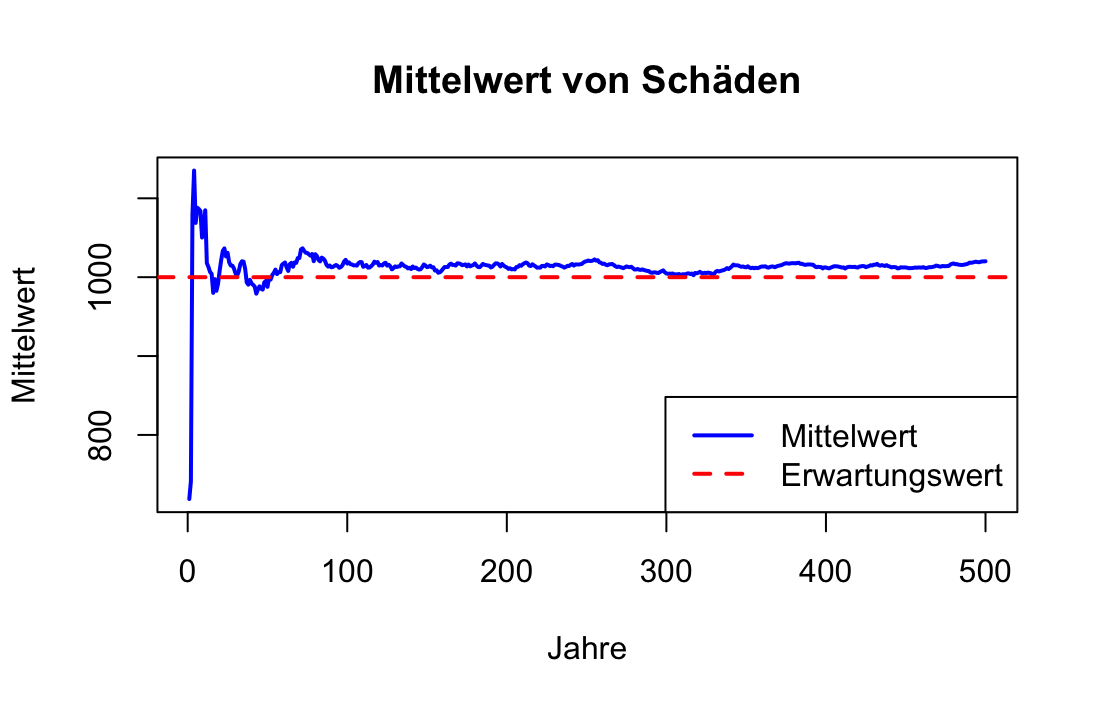
\includegraphics[width=0.9\textwidth]{schaden.png}
  \caption{Simulation des Mittelwertes eines Schadens}
  \label{fig:schaden}
\end{figure}

Anhand dessen können z.B. Versicherungsprämien stabil und planbar berechnet werden. Die Planbarkeit ist vor allem bei großen internationalen Firmen von großer Bedeutung, besonders wenn das Unternehmen börsennotiert ist und Aktionäre sowie Analysten bestimmte Erwartungen gegenüber dem Unternehmenserfolg haben.


\subsection{Monte-Carlo-Simulationen}

Das GGZ stellt die grundlegende theoretische Basis für das Monte-Carlo-Verfahren dar.
Bei diesem Verfahren wird der Erwartungswert von Zufallsvariablen durch Mittelung über Simulationen angenähert.
Wenn \( X_1, X_2, \dots, X_n \sim \text{i.i.d.} \) mit Erwartungswert \( \mu \) sind, dann gilt
\[
\frac{1}{n} \sum_{i=1}^n f(X_i) \xrightarrow{\mathbb{P}} \mathbb{E}[f(X)].
\]
Somit ermöglichen Monte-Carlo-Simulationen stochastische Optimierungen  \citep{degroot2021}.


\begin{figure}[h!]
  \centering
  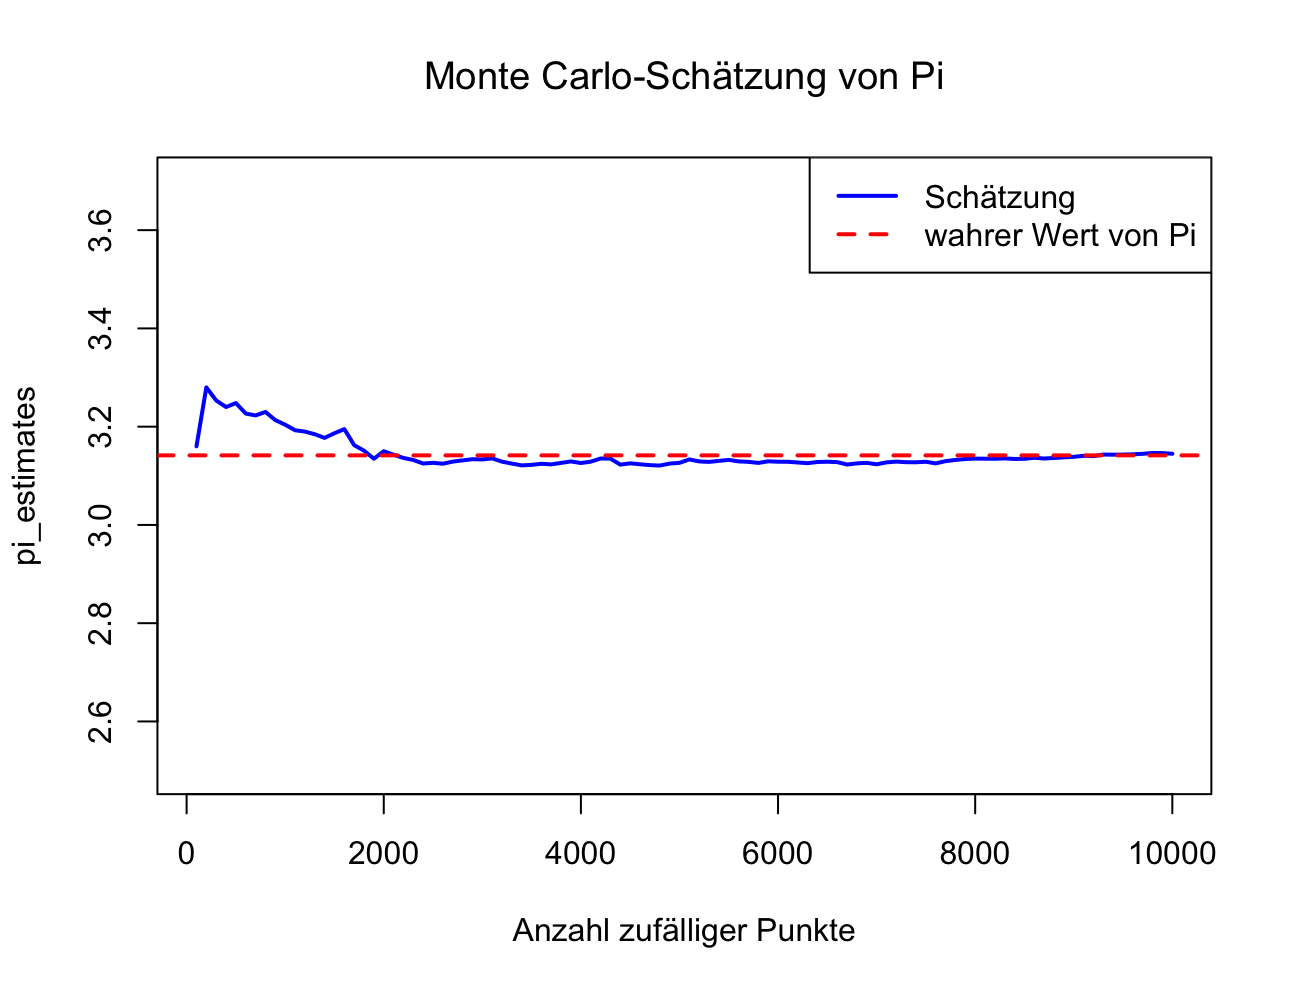
\includegraphics[width=0.9\textwidth]{Monte_carlo.png}
  \caption{Monte-Carlo-Simulation zur Schätzung des wahren Wertes von \texorpdfstring{$\pi$}{π}}
  \label{fig:monte_carlo}
\end{figure}


Beispielsweise kann man eine Monte-Carlo-Simulation durchführen, um den wahren Wert von \texorpdfstring{$\pi$}{π} analytisch zu schätzen.
Dabei werden zufällige Punkte in einem Einheitsquadrat generiert und geprüft, ob sie im Viertelkreis mit Radius 4 liegen.
Je mehr Punkte man generiert, desto näher wird der Anteil der Punkte in diesem Viertelkreis an dem wahren Wert von \texorpdfstring{$\pi$}{π} liegen.
Die Ergebnisse dieser Simulation in der Programmiersprache R sieht man in Abbildung \ref{fig:monte_carlo}.
Wie man grafisch beobachten kann, nähert sich die Monte-Carlo-Schätzung an den wahren Wert von \texorpdfstring{$\pi$}{π}, wenn man die Anzahl der Zufallspunkte erhöht.
Anhand dieses Programmierbeispiels sieht man gut, wie das GGZ praktisch angewendet werden kann, um bestimmte mathematische Problemstellungen zu lösen.


\subsection{Wirtschaft}


In der Volkswirtschaftslehre und Finanzwissenschaft beschreibt das GGZ die Verlässlichkeit von Aggregatgrößen.
Zum Beispiel kann durch die Aggregation individueller Einkommen oder Konsumentscheidungen über viele zeitliche oder örtliche Einheiten hinweg das durchschnittliche Verhalten der Bevölkerung mit hoher Genauigkeit approximiert werden.
Diese Annäherung ist von großer Bedeutung in der Volkswirtschaftslehre und Makroökonomie, weil es oft praktisch unmöglich ist, die gesamte Bevölkerung zu bestimmten Themen zu befragen.


\section{Gegenbeispiele und Grenzen des Gesetz der Großen Zahlen}
\label{sec:grenzen}


\subsection{Das schwache Gesetz der großen Zahlen}


Das schwache und das starke GGZ sind fundamentale Sätze in der Mathematik, die eine Art Stabilisierung des Mittelwertes bei einer steigenden Anzahl von Wiederholungen eines Zufallsexperiments beschreiben.
Trotz ihrer grundlegenden Bedeutung und ihrer breiten Anwendung in der Praxis sind beide Gesetze in manchen Fällen nur mit bestimmten Einschränkungen oder überhaupt nicht anwendbar.
In diesem Kapitel werden Gegenbeispiele und Grenzen beider Gesetze präsentiert, um ihre Gültigkeit und die Bedingungen, unter denen sie gelten, näher zu untersuchen.


Ein klassischer Fall, in dem das schwache GGZ nicht gilt, betrifft Zufallsvariablen, die nicht identisch verteilt sind.
Wenn die Variablen nicht identisch verteilt sind, kann der Mittelwert nicht mit Wahrscheinlichkeit 1 gegen den Erwartungswert konvergieren, selbst wenn der Erwartungswert existiert.
Ein solches Beispiel wird in der Verallgemeinerung der \textit{Bernstein'schen Ungleichung} dargestellt.
Angenommen, es gibt eine Folge von Zufallsvariablen \(X_1, X_2, \dots, X_n\), die nicht identisch verteilt sind, aber jeweils einen endlichen Erwartungswert \(\mu_i = \mathbb{E}[X_i]\) und eine endliche Varianz \(\sigma_i^2 = \text{Var}(X_i)\) haben. Die Bernstein'sche Ungleichung für die Verallgemeinerung dieser Zufallsvariablen lautet:
\[
\mathbb{P}\left( \left|\frac{1}{n} \sum_{i=1}^n X_i - \mu \right| \geq \epsilon \right) \leq 2 \exp \left( -\frac{n \epsilon^2}{2 \sum_{i=1}^n \sigma_i^2 + \frac{3}{2} \epsilon \sum_{i=1}^n |X_i - \mu_i|} \right)
\]

Diese Ungleichung zeigt also, dass für nicht identisch verteilte Zufallsvariablen die Wahrscheinlichkeit, dass der Mittelwert von den erwarteten Werten abweicht, exponentiell mit einer Kombination von Varianzen und Abweichungen der Zufallsvariablen selbst sinkt.
Trotzdem kann vorkommen, dass die Konvergenz sehr langsam oder überhaupt nicht passiert, wenn die Varianzen \(\sigma_i^2\) oder die Abweichungen \(|X_i - \mu_i|\) zu groß sind \citep{stoyanov2013}.


Ein weiteres wichtiges Gegenbeispiel für das schwache GGZ ist der Fall abhängiger Zufallsvariablen.
Gegeben eine abhängige Struktur von Zufallsvariablen \(X_1, X_2, \dots\), wie z.B. eine autoregressive Struktur:

\[
X_n = \alpha X_{n-1} + \epsilon_n \quad \text{mit} \quad \epsilon_n \sim \mathcal{N}(0, \sigma^2)
\]

In diesem Fall, selbst wenn die \(X_n\) Zufallsvariablen identisch verteilt sind und einen Erwartungswert von \(\mu = 0\) haben, kann der Mittelwert nicht gegen \(\mu\) konvergieren.

Grund dafür ist die Abhängigkeit zwischen den Zufallsvariablen. Ist zum Beispiel \(X_1 = X_2 = \dots = X_n = Z\) für eine Zufallsvariable \(Z\), so ist auch der Mittelwert gleich \(\bar{X}_n = Z\). In diesem Fall ändert sich der Mittelwert mit wachsendem \(n\) gar nicht, sondern bleibt eine Zufallsvariable (\(Z\)) mit fester Varianz. Es gilt dann:
\[
\text{Var}(\bar{X}_n) = \text{Var}(Z),
\]
während bei unabhängigen Zufallsvariablen mit Varianz \(\sigma^2\) gilt:
\[
\text{Var}(\bar{X}_n) = \frac{\sigma^2}{n} \to 0 \quad \text{für } n \to \infty.
\]
Ohne Unabhängigkeit verschwindet also die Streuung des Mittelwerts nicht mit wachsendem Stichprobenumfang.
Damit wird auch nicht garantiert, dass \(\bar{X}_n\) mit hoher Wahrscheinlichkeit nahe bei \(\mu\) liegt.
Die Konvergenz in Wahrscheinlichkeit (wie sie das schwache Gesetz der großen Zahlen fordert) kann daher fehlschlagen.
Dies sieht man auch in Abbildung \ref{fig:ar1}, wo ein AR(1)-Prozess mit 1000 Zeitpunkten und 50 verschiedenen Pfaden simuliert wurde.
Der Plot zeigt das Verhalten von Stichprobenmittelwerten bei stark abhängigen Zufallsvariablen mit einem Autokorrelationsparameter von 0.9.
Hier sieht man, dass zwar alle Prozesse denselben Erwartungswert haben, führt die starke Autokorrelation dazu, dass die Mittelwerte auch bei großen Stichprobenumfängen nicht konvergieren, wie es das schwache GGZ verlangen würde.


\begin{figure}[h!]
  \centering
  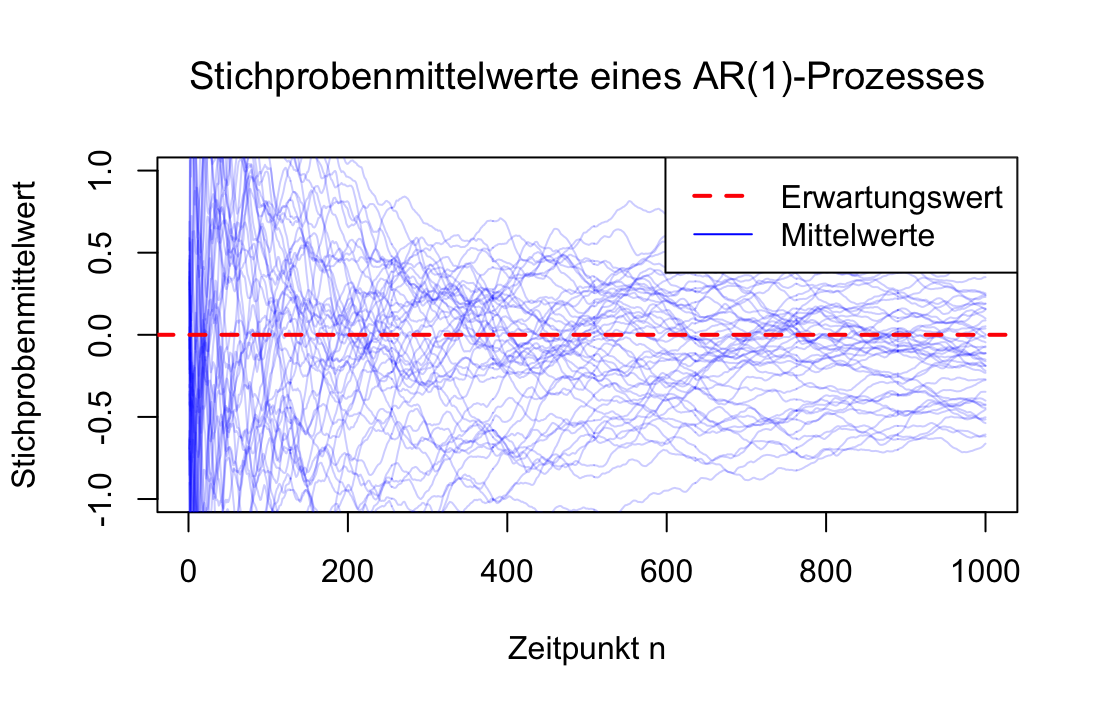
\includegraphics[width=0.9\textwidth]{ar1.png}
  \caption{Stichprobenmittelwerte eines AR(1)-Prozesses}
  \label{fig:ar1}
\end{figure}


Man sieht also, dass sowohl die Annahme für \textbf{identisch} als auch für \textbf{unabhängig} verteilte Zufallsvariablen wichtig ist, damit das schwache (und somit auch das starke) GGZ gilt.
Jedoch muss man bei praktischen Anwendungen oft berücksichtigen, dass diese Annahmen nicht alle erfüllt werden können.
Beispielsweise bei Finanzdaten, wie Aktienkursen oder Wechselkursen sind die Datenpunkte zeitlich voneinander abhängig (Autokorrelation), wodurch das GGZ nicht korrekt angewendet werden kann.
Ähnlich ist es auch z.B. bei Umweltdaten, wie Temperatur oder Niederschlag.
Hier sind Messpunkte oft nicht (nur) zeitlich, sondern auch räumlich voneinander abhängig.
Daher gelten meistens Konvergenzgesetze wie das GGZ standardmäßig nicht.


\subsection{Das starke Gesetz der großen Zahlen}


Ein berühmtes Gegenbeispiel für das starke GGZ ist die \textit{Cauchy-Verteilung}, die in der Mathematik oft als Beispiel für unendliche Varianz verwendet wird. Die Dichtefunktion der Cauchy-Verteilung wird folgenderweise definiert.

\[
f(x) = \frac{1}{\pi (1 + x^2)}
\]

Variablen mit einer Cauchy-Verteilung haben keinen endlichen Erwartungswert und keine endliche Varianz.
Das starke GGZ besagt jedoch, dass für eine Folge von i.i.d. Zufallsvariablen \( X_1, X_2, \dots \) mit \textit{endlichem} Erwartungswert und \textit{endlicher} Varianz folgender Zusammenhang gilt.

\[
\frac{1}{n} \sum_{i=1}^n X_i \xrightarrow{a.s.} \mu \quad \text{für} \quad \mu = \mathbb{E}[X_i]
\]

Für die Cauchy-Verteilung existiert aber \(\mathbb{E}[X_i]\) nicht, und somit kann das starke GGZ keine fast sichere Konvergenz garantieren.
Ähnlicherweise, wenn die Zufallsvariablen eine unendliche Varianz besitzen, können ihre Mittelwerte nicht mit Wahrscheinlichkeit 1 gegen einen festen Wert konvergieren.
Somit ist die Cauchy-Verteilung der Zufallsvariablen ein Gegenbeispiel für sowohl das starke als auch das schwache GGZ.


Ein weiteres Gegenbeispiel für das starke GGZ ist die Normalverteilung der Zufallsvariablen. Gegeben sei eine Folge von i.i.d. normalverteilten Zufallsvariablen \( X_1, X_2, \dots \) mit Erwartungswert \(\mu\) und Varianz \(\sigma^2\). Dann gilt für diese Zufallsvariablen

\[
\frac{1}{n} \sum_{i=1}^n X_i \xrightarrow{a.s.} \mu
\]

Die Konvergenz ist also garantiert, sie kann jedoch sehr langsam erfolgen.
Dies liegt nicht daran, dass die Zufallsvariablen normalverteilt sind, sondern an der Größe der Varianz \(\sigma^2\): Ist diese groß, so bleibt auch die Streuung des Mittelwerts über viele Stichproben hinweg deutlich, insbesondere bei kleinen Werten von \(n\).

Anhand des zentralen Grenzwertsatzes wissen wir, dass der Mittelwert
\[
\bar{X}_n = \frac{1}{n} \sum_{i=1}^n X_i
\]
näherungsweise normalverteilt ist mit
\[
\text{Var}(\bar{X}_n) = \frac{\sigma^2}{n}.
\]
Ist \(\sigma^2\) groß, so ist auch \(\text{Var}(\bar{X}_n)\) für kleine \(n\) noch groß. In solchen Fällen können signifikante Abweichungen von \(\mu\) auftreten, obwohl die Konvergenz gegen \(\mu\) im Grenzwert gesichert ist. Dieses Verhalten des Mittelwerts bei endlichem \(n\) lässt sich also direkt durch seine Varianz erklären.


Dadurch sieht man, dass die Konvergenz für Zufallsvariablen mit solcher Verteilung zwar existiert, aber sehr langsam sein kann.
Anhand des zentralen Grenzwertsatzes wissen wir, dass die Geschwindigkeit der Konvergenz so niedrig sein kann, dass der Mittelwert eventuell über kleine Stichprobengrößen noch immer signifikante Abweichungen von \(\mu\) aufweist.
Dieses Verhalten des Mittelwerts kann man mit folgender Varianzformel für den Mittelwert der \(n\) Zufallsvariablen näher betrachten.

\[
\text{Var}\left( \frac{1}{n} \sum_{i=1}^n X_i \right) = \frac{\sigma^2}{n}
\]

Mithilfe der Formel sieht man, dass die Varianz zwar mit wachsendem \(n\) sinkt.
Jedoch erfolgt die Konvergenz in der Praxis sehr langsam, wodurch das starke GGZ in vielen Anwendungsfällen nicht zielführend verwendet werden kann, weil sich der Mittelwert nicht innerhalb einer realistischen Stichprobengröße stabilisiert.


Wie bereits beschrieben, ist das starke GGZ strenger als das schwache Gesetz.
Anders gesagt, garantiert das starke Gesetz eine fast sichere Konvergenz, während das schwache Gesetz lediglich eine Konvergenz in Wahrscheinlichkeit garantiert.
Die unterschiedlichen Konvergenzen und Voraussetzungen führen dazu, dass beide Gesetze in der Praxis anders verwendet werden.


\section{Zusammenfassung}
\label{sec:zusammenfassung}


Das Gesetz der großen Zahlen ist ein fundamentales Ergebnis in der Mathematik, das vor mehreren Jahrhunderten etabliert wurde und mittlerweile in diversen Anwendungsfällen verwendet wird.
Es besagt die Stabilität in stochastischen Systemen und Prozessen und liefert die theoretische Grundlage für viele weitere Methoden in verschiedenen Bereichen.
Es erklärt, warum durchschnittliches Verhalten verlässlich ist, obwohl einzelne Beobachtungen zufällig sind.
Diese Aussage ist äußerst relevant, wenn man mit großen Datenmengen arbeitet und die Analyse jeder einzelnen Beobachtung praktisch unmöglich ist.
Für die Zwecke dieser Arbeit wurde auch der Unterschied zwischen dem starken und schwachen GGZ veranschaulicht.
Dieser liegt hauptsächlich in der Art der Konvergenz.
Das schwache GGZ besagt eine Konvergenz in Wahrscheinlichkeit, während das starke GGZ eine fast sichere Konvergenz garantiert.
Dadurch trifft das starke GGZ eine stärkere Aussage, und dementsprechend gilt das schwache GGZ immer, wenn das starke GGZ gilt, aber nicht umgekehrt.
Einige Beispiele für diesen Zusammenhang werden in \citet{stoyanov2013} diskutiert.


Diese Arbeit beschränkt sich auf die theoretische Darstellung und den historischen Kontext des GGZ.
Es wurde jedoch keine empirische Untersuchung zur Veranschaulichung der Konvergenzeigenschaften durchgeführt und somit keine eigenen Daten gesammelt.
Darüber hinaus wurde hier nicht auf einzelne Verallgemeinerungen und Ausnahmen eingegangen.
Aus diesen Einschränkungen ergeben sich aber zahlreiche Möglichkeiten für weitere Forschung.
Beispielsweise könnte sich zukünftige Forschung näher mit der Anwendung des GGZ unter realitätsnäheren Bedingungen beschäftigen.
Beispielsweise sind Zeitreihenanalysen in Bezug auf das GGZ in den Finanzwissenschaften von großer Bedeutung.
Weiters könnten auch quantitative Merkmale des GGZ, wie z.B. die Geschwindigkeit der Konvergenz, näher analysiert werden, um die praktische Anwendbarkeit des GGZ detailliert zu untersuchen.

\newpage

%========= Appendix ==========

\appendix


\section{Appendix section}
\label{sec:app}

\textbf{R-Code zur Simulation von Münzwürfen}

\begin{lstlisting}[language=R, caption={Simulation von Münzwürfen mit R}, label={lst:muenzenwurf}]
n <- 10000
set.seed(123)
w <- rbinom(n, size = 1, prob = 0.5)
m <- cumsum(w) / 1:n
e <- 0.5
plot(1:n, m, type = "l", col = "blue",
     xlab = "Anzahl der Wuerfe",
     ylab = "Empirischer Mittelwert",
     main = "Beispiel: Muenzwurf")
abline(h = e, col = "red", lty = 2)
legend("topright", legend = c("Empirischer Mittelwert", "Erwartungswert (0.5)"),
       col = c("blue", "red"), lty = c(1,2), bty = "n")
\end{lstlisting}

\textbf{R-Code zur Schätzung von \texorpdfstring{$\pi$}{π}}

\begin{lstlisting}[language=R, caption={Monte-Carlo-Schaetzung von $\pi$ mit R}, label={lst:pi_montecarlo}]
n <- 10000
schritt <- 100
x <- runif(n)
y <- runif(n)
ist_drinnen <- x^2 + y^2 <= 1
pi <- numeric(n / schritt)
for (i in seq(schritt, n, by = schritt)) {
  pi[i / schritt] <- 4 * mean(ist_drinnen[1:i])
}
x_werte <- seq(schritt, n, by = schritt)
plot(x_werte, pi, type = "l", col = "blue", lwd = 2,
     main = expression("Monte Carlo-Schaetzung von Pi"),
     xlab = "Anzahl zufaelliger Punkte",
     ylim = c(2.5, 3.7))
abline(h = pi, col = "red", lty = 2, lwd = 2)
legend("topright", legend = c("Schaetzung", "wahrer Wert von Pi"),
       col = c("blue", "red"), lty = c(1, 2), lwd = 2)
\end{lstlisting}

%====== References ========

\newpage
\bibliographystyle{imsart-nameyear}
\bibliography{literatur}


\end{document}